\documentclass{ctexart}
\usepackage{amsmath}
\usepackage{graphicx}
\title{4.2 特殊矩阵变换和运算}
\author{翻译:fangcun}
\begin{document}
\maketitle
\newpage
\tableofcontents
\newpage
本章节介绍一些实时渲染用到的矩阵变换和运算。首先,我们介绍\textbf{Euler}变换(以及它的参数提取),它可以非常直观地描述方位。接着,我们介绍如何从一个矩阵
提取一系列的基本变换。最后,我们导出围绕任意轴旋转实体的方法。

\section{4.2.1 Euler变换}
\textbf{Euler}变换是一个非常直观的构造\textbf{描述方位}矩阵的方法(可以用它来实现相机)。它的名字来自伟大的科学家\textbf{Euler}。

\begin{figure}
	\centering
	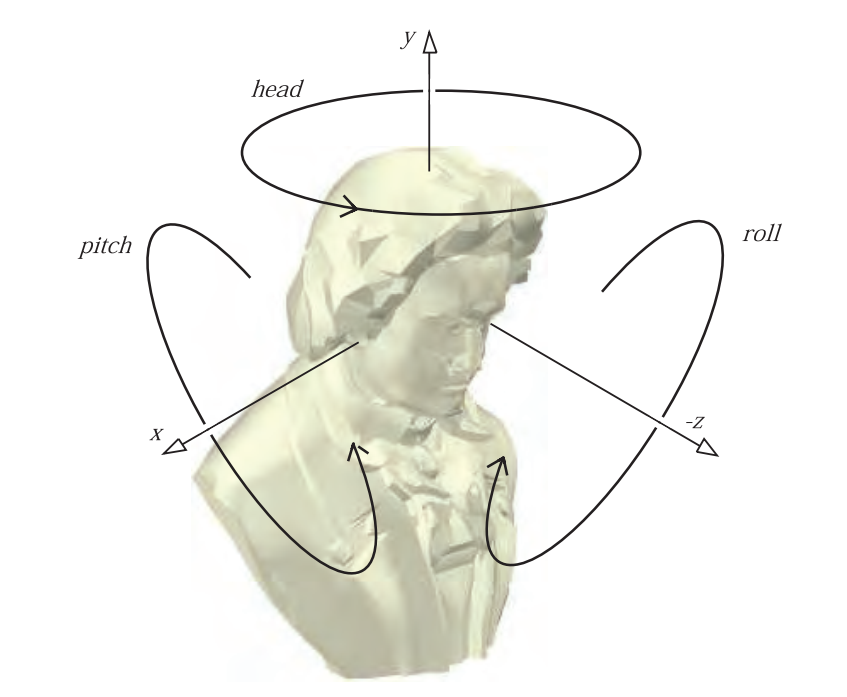
\includegraphics[scale=0.8]{4-6.png}
	\caption{插图形象地描述了\textbf{Euler}变换,它由$head$,$pitch$和$roll$构成方位。缺省视图下,观察方向沿着$z$轴负方向,头部绕$y$轴。}
	\label{EulerFigure}
\end{figure}

首先,我们建立一个缺省的视图。大多数情况下,我们使用图\ref{EulerFigure}这样的视图作为缺省视图。\textbf{Euler}变换是由三个旋转矩阵构成的,它们的名字
已经在图\ref{EulerFigure}中给出。下面给出它的更正规的定义,
我们使用$E$来表示\textbf{Euler}变换,它由公式\ref{EulerEqu}给出。

\begin{equation}
	\label{EulerEqu}
	E(h,p,r)=R_{z}(r)R_{x}(p)R_{y}(h)
\end{equation}

因为$E$是由旋转构成的,所以显然它是正交的。正交矩阵的逆就是它本身的转置,
所以$E^{-1}=E^{T}=(R_{z}R_{x}R_{y})^{T}=R_{y}^{T}R_{x}^{T}R_{z}^{T}$,通常,我们直接使用转置运算来求$E$的逆。

\textbf{Euler}角$h$,$p$和$r$表示旋转的顺序以及旋转的程度。
\textbf{Euler}变换非常直观,在和外行人讨论时使用它,很容易被人理解。
比如,改变$head$角度就是让观察者转动他的头说"no",改变$pitch$角度,就是
让他点头,$roll$则使他的头向一边倾斜。相比于,使用绕$x$,$y$,$z$轴旋转,
使用这种方式显然更加直观。\textbf{Euler}变换不仅可以使用在相机上,还
可以使用在其它物体上。它可以使用在世界坐标系或相对于一个局部的参照物来使用。

使用\textbf{Euler}变换,可能会导致万向节锁。当进行旋转操作造成一个维度
消失时就会出现。比如,我们进行变换的顺序是$x/y/z$。考虑第二次旋转时围绕$y$轴旋转$\pi/2$。执行后,$z$轴现在在原来$x$轴的位置,第三次围绕$z$轴的变换变的多余。

\begin{equation}
	\label{GImbalLock}
	\begin{split}
	E(h,\pi/2,r)&=
	\left(
		\begin{array}{ccc}
			cosrcosh-sinrsinh & 0 & cosrsinh+sinrcosh\\
			sinrcosh+cosrsinh & 0 & sinrsinh-cosrcosh\\
			0                 & 1 &                 0\\
		\end{array}
	\right)\\
	&=
	\left(
	\begin{array}{ccc}
	cos(r+h) & 0 & sin(r+h)\\
	sin(r+h) & 0 & -cos(r+h)\\
	0 & 1 & 0\\
	\end{array}
	\right)
	\end{split}
\end{equation}

我们可以看到这个矩阵只依赖了$r+h$,由此,我们可以推断我们已经失去了一个维度。

尽管\textbf{Euler}角在模型系统中通常使用$x/y/z$顺序表示,但其它顺序也是可行的。比如,$z/x/y$经常被使用在动画中,$z/x/z$在动画和物理中都经常被使用。
它们都是有效的指定三个独立旋转的方法。$z/x/z$顺序非常适合一些程序,

尽管\textbf{Euler}角对于小范围的角度改变很有用,但它还是有一些严重的限制。
比如,我们很难将两个不同的\textbf{Euler}角进行组合使用。两个不同的\textbf{Euler}角可能定义相同的方位,对它们两者进行插值不应该产生任何旋转。这也是使用
其它替代方式,比如四元数来表示方位的原因。我们将在后面的章节讨论四元数。

\section{4.2.2 从Euler变换中导出参数}

有时,我们需要从一个正交矩阵中导出\textbf{Euler}参数$h$,$p$和$r$。导出的方法由公式\ref{Mat2EulerP}给出。

\begin{equation}
	\label{Mat2EulerP}
	F=\left(
	\begin{array}{ccc}
		f_{00} & f_{01} & f_{02}\\
		f_{10} & f_{11} & f_{12}\\
		f_{20} & f_{21} & f_{22}\\
	\end{array}
	\right)=R_{z}(r)R_{x}(p)R_{y}(h)=E(h,p,r)
\end{equation}

我们把三个矩阵连乘后的结果放入相应项目中得到公式\ref{Mat2EulerP2}。

\begin{equation}
	\label{Mat2EulerP2}
	F=\left(
	\begin{array}{ccc}
		cosrcosh-sinrsinpsinh & -sinrcosp & cosrsinh+sinrsinpcosh\\
		sinrcosh+cosrsinpsinh & cosrcosp  & sinrsinh-cosrsinpcosh\\
		-cospsinh			  & sinp	  & cospcosh
	\end{array}
	\right)
\end{equation}

显然我们可以从$sinp=f_{21}$得到$pitch$参数。同样,通过$f_{01}$除以
$f_{11}$和$f_{20}$除以$f_{22}$可以得到$head$和$roll$参数。

\begin{equation}
	\label{ExtEuler1}
	\begin{split}
		&\frac{f_{01}}{f_{11}}=\frac{-sinr}{cosr}=-tanr\\
		&\frac{f_{20}}{f_{22}}=\frac{-sinh}{cosh}=-tanh\\
	\end{split}
\end{equation}

至此,我们就从矩阵$F$中到导出了\textbf{Euler}参数$h$(head),$p$(pitch)和
$r$(roll),公式\ref{ExtEuler2}给出了这一过程。

\begin{equation}
	\label{ExtEuler2}
	\begin{split}
		&h=\textbf{atan2}(-f_{20},f_{22})\\
		&p=arcsin(f_{21})\\
		&r=\textbf{atan2}(-f_0={01},f_{11})\\
	\end{split}
\end{equation}

实际上,还有一个地方我们需要处理。当$cosp=0$时,$f_{01}=f_{11}=0$,
$\textbf{atan2}$函数就不能使用了,但是$cosp=0$意味着$sinp=\pm 1$,所以此时$F$可以
简化为:

\begin{equation}
	\label{ExtEuler3}
	F=\left(
		\begin{array}{ccc}
			cos(r\pm h) &   0   & sin(r\pm h)\\
			sin(r\pm h) &   0   & -cos(r\pm h)\\
			0			&  \pm 1& 			 0\\
		\end{array}
	\right)
\end{equation}

现在我们设置$h=0$,那么可以得到$sinr/cosr=tan=f_{10}/f_{00}$,
从而得到$r=\textbf{atan2}(f_{10},f_{00})$。

\section{4.2.3 矩阵分解}

到现在为止,我们知道我们使用的矩阵是如何经过变换产生的,但这种情况在实际工作中并不普遍,有时,我们需要从一个矩阵获取不同的变换信息,这时就需要进行
\textbf{矩阵分解}。

有许多情况需要我们这样做,包括:

\begin{itemize}
	\item 导出对象的缩放系数。
	\item 为一个特别的系统提供变换。比如VRML使用\emph{Transform}节点进行变换,不能使用4x4矩阵。
	\item 确定一个模型是否只经过了刚体变换。
	\item 需要对关键帧进行插值,但只有对象的矩阵可以使用。
	\item 移除旋转矩阵中的错切。
\end{itemize}

\section{4.2.4 关于任意轴旋转}

可以绕任意轴旋转实体有时是非常便利的。现在假设旋转轴$r$是规范化的,我们需要旋转的角度是$\alpha$。

首先我们找到和$r$互相垂直的另外两个单位长度的轴。它们三者组成了一个坐标基。

\begin{figure}
	\centering
	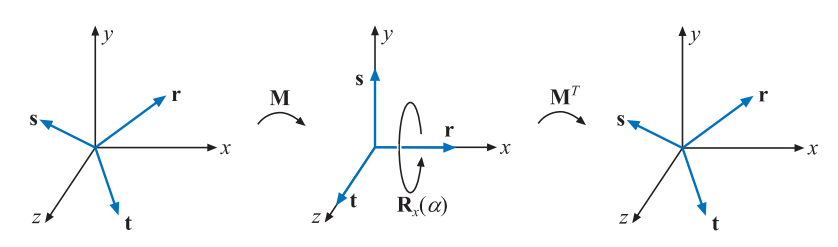
\includegraphics[scale=0.8]{4-7.png}
	\caption{首先找到由$r$,$s$和$t$构成的正交基,然后通过变换将这个正交基和标准基对齐,使$r$和$x$轴对齐,之后绕$x$轴旋转,最后再变换回去。}
	\label{EulerFigure}
\end{figure}

第一步,我们需要计算坐标基。我们已经有了一个轴$r$,也就是我们需要围绕
旋转的轴。接着,我们需要找$s$和$t$。显然$t=r\times s$。一个数值稳定的
方法是找$r$的绝对值最小的分量,然后将这个分量设置为0,交换另外两个分量的位置,最后将这两个分量交换位置后的第一个取相反数。整个过程的数学表示如公式\ref{RotateArb1}。

\begin{equation}
	\label{RotateArb1}
	\begin{split}
	&\bar{s}=\left\{
		\begin{array}{cc}
			(0,-r_{z},z_{y}) &if\quad |r_{x}|<|r_{y}|\quad and\quad|r_{x}|<|r_{z}|\\
			(-r_{z},0,r_{x}) &if\quad |r_{y}|<|r_{x}|\quad and\quad |r_{y}|<|r_{z}|\\
			(-r_{y},r_{x},0) &if\quad |r_{z}|<|r_{x}|\quad and\quad |r_{z}|<|r_{y}|\\
		\end{array}
	\right.\\
	&s=\bar{s}/||\bar{s}||\\
	&t=r\times s\\
	\end{split}
\end{equation}

这保证$\bar{s}$和$r$正交(垂直),$(r,s,t)$构成了一个正交基。我们使用三个向量构成一个矩阵$M$,如
公式\ref{RotateArb2}。

\begin{equation}
	\label{RotateArb2}
	\begin{split}
		M=\left(
			\begin{array}{c}
				r^T\\
				s^T\\
				t^T\\
			\end{array}
		\right)
	\end{split}
\end{equation}

这个矩阵将向量$r$变换到$x$轴,$s$变换到$y$轴,$t$变换到$z$轴。最后关于规范化向量$r$旋转$\alpha$
弧度的变换如公式\ref{RotateArb3}所示。

\begin{equation}
	\label{RotateArb3}
	X=M^TR_{x}(\alpha)M
\end{equation}

也就是说,首先我们把$r$变换到$x$轴(使用$M$),然后绕$x$轴旋转 $\alpha$ 弧度(使用$R_x(\alpha)$),
最后我们使用$M$的逆矩阵变换回去,由于$M$是正交的,所以$M^T$就是它的逆。

另一个绕任意轴旋转的方法,由Gloadman提出。这里,我们直接给出他的变换,如公式\ref{RotateArb4}。

\begin{equation}
	\label{RotateArb4}
	R=\left(
		\begin{array}{ccc}
			cos\phi+(1-cos\phi)r_{x}^{2} & (1-cos\phi)r_{x}r_{y}-r_{z}sin\phi & (1-cos\phi)r_{x}r_{z}+r_{y}sin\phi\\
			(1-cos\phi)r_{x}r_{y}+r_{z}sin\phi & cos\phi+(1-cos\phi)r_{y}^2 & (1-cos\phi)r_{y}r_{z}-r_{x}sin\phi\\
			(1-cos\phi)r_{x}r_{z}-r_{y}sin\phi & (1-cos\phi)r_{y}r_{z}+r_{x}sin\phi &
			cos\phi+(1-cos\phi)r_{z}^{2}\\
		\end{array}
	\right)
\end{equation}

在章节4.3.2,我们给出解决这个问题的另一个方法,使用四元数,且它解决相关问题的效率更高,比如从一个向量旋转到另一个向量的问题。

\end{document}